\documentclass{article}

\usepackage{graphicx}
\usepackage{multicol}
\usepackage{matlab-prettifier}
\usepackage{graphicx}
\usepackage{subcaption}
\usepackage{float}
\usepackage{verbatimbox}
\usepackage{amssymb}
\usepackage{amsmath}
\usepackage{epstopdf}

\usepackage{tikz}
\usepackage{pgfplots}

% For drawing circuits
\usepackage{circuitikz}
\ctikzset {bipoles/length=1.2cm}

\pgfplotsset{compat=newest}
\usepgfplotslibrary{units}
\usetikzlibrary{plotmarks}

% decrease all margins
\addtolength{\oddsidemargin}{-1cm}
\addtolength{\evensidemargin}{-1cm}
\addtolength{\textwidth}{2cm}

% definition to control the margins for a given part of text
\def\changemargin#1#2{\list{}{\rightmargin#2\leftmargin#1}\item[]}
\let\endchangemargin=\endlist

% all matlab code should appear numbered and with a left line separating line numbers from code
\lstset{numbers = left, frame=single}

% graphics are in 'images' folder
\graphicspath{{./images/}}

% useful for development
\usepackage{color}

% creates an environment for displaying hypotheses------------------------------------
\usepackage[many]{tcolorbox}
\usepackage{enumitem}
\usepackage{amsmath,amssymb}
\newcounter{myhypo}
\renewcommand\themyhypo{(H\arabic{myhypo})} % How the labeling is going to be made
\newtcolorbox{hypo}[1][]{
  breakable,
  enhanced,
  top=0pt,
  bottom=0pt,
  nobeforeafter,
  colback=white,
  boxrule=0pt,
  arc=0pt,
  right=30pt,
  left=20pt,
  outer arc=0pt,
  overlay={
    \node[inner sep=0pt,anchor=east]
    at (frame.east)
    {\refstepcounter{myhypo}\themyhypo\label{#1}};
  },
}
\newenvironment{hypotheses}
  {\list{}{\setlength\leftmargin{0pt}\item\relax}}
  {\endlist}
\newcommand\Hypo[2][]{%
  \begin{hypo}[#1]#2\end{hypo}}
% ----------------------------------------------------------------------------------







\begin{document}

    \newpage

%    Primeiramente vamos definir o sistema de interesee. O que que vamos analisar de fato. Modelo matemático do que?
%
%    Vamos desenvolver o modelo matemático para um BLDC.
%
%    Algumas hipóteses simplificadoras foram feitas, para viabilizar a modelagem
    \begin{hypotheses}
        \Hypo[hyp:same_R]{All of the phases of the BLDC have the same resistance}
        \Hypo[hyp:same_L]{All of the phases of the BLDC have the same inductance}
        \Hypo[hyp:constant_airgap]{The airgap length is constant}
        \Hypo[hyp:rigid_bodies]{All of the components in the mechanical subsystem are rigid bodies}
        \Hypo[hyp:friction_model]{The friction torque acting on the shaft of the motor is composed of viscous friction (proportional to the angular velocity) and Coulomb friction}
        \Hypo[hyp:mutual_inductances_negligible]{The mutual inductances are negligible \textcolor{red}{improve this sentence}...}
        \Hypo[hyp:bemf_proportional_omega]{The back emf in each phase is proportional to the angular velocity of the motor}
    \end{hypotheses}
    \quad

%    Para fazer um modelo desse sistema, começamos quebrando ele em dois subsistemas mais simples. Um subsist mecanico e um elétrico. O susbsitema elétrico é a parte elétrica mesmo, cuja entrada é a tensão em cada uma das bobinas e a saída é o torque que será aplicado no eixo do motor. O subsistema elétrico é a parte mecânica do motor, relacionada ao movimento do eixo; é o subsistema cuja entrada é o torque aplicado no eixo e a saída é a velocidade angular do eixo do motor. A seguir cada um dos subsistemas será analisado mais aprofundadamente.


    \subsection{Electrical subsystem analysis}
    \label{sec:elec_subsystem}

     A diagram of the electrical subsystem is shown in figure \ref{fig:electrical_subsys}, assuming \ref{hyp:same_R} and \ref{hyp:same_L}. From it, it's possible to obtain expressions for $v_{ab}$, $v_{bc}$ and $v_{ca}$ (defined as $v_a-v_b$, $v_b-v_c$ and $v_c-v_a$, respectively) [\textcolor{red}{citation needed}]. That, added to the fact that the currents in each phase must sum to zero (Kirchhoff's current law in the central node) and \ref{hyp:mutual_inductances_negligible}, leads to the following equations:

    \begin{figure}[H]
        \center
        \newcommand{\myvar}{1.8}
        \begin{circuitikz}[scale=0.6, every node/.style={scale=1}]
            \ctikzset{label/align = straight}
            \draw

            % Phase a
            (0,3*\myvar) to [R=$R$] (0,2*\myvar) to [american voltage source, l_=$e_a$] (0,1*\myvar) to [inductor, l=$L$, -*] (0,0)
            (0,3*\myvar+1) to [short,i=$i_a$, o-] (0,3*\myvar)
            (0,3*\myvar+1) node[anchor=south]{$a$}

            % Phase b
            (-\myvar*3*0.866,-\myvar*3/2) to [R=$R$] (-\myvar*2*0.866,-\myvar*2/2) to [american voltage source, l=$e_b$] (-\myvar*0.866,-\myvar/2) to [inductor, l=$L$] (0,0)
            (-\myvar*3*0.866-1*0.866,-\myvar*3/2-1/2) to [short, i=$i_b$,o-] (-\myvar*3*0.866,-\myvar*3/2)
            (-\myvar*3*0.866-1*0.866,-\myvar*3/2-1/2) node[left]{$b$}

            % Phase c
            (\myvar*3*0.866,-\myvar*3/2) to [R,l_=$R$] (\myvar*2*0.866,-\myvar*2/2) to [american voltage source, l_=$e_c$] (\myvar*0.866,-\myvar/2) to [inductor, l,l_=$L$] (0,0)
            (\myvar*3*0.866+1*0.866,-\myvar*3/2-1/2) to [short,i=$i_c$,o-] (\myvar*3*0.866,-\myvar*3/2)
            (\myvar*3*0.866+1*0.866,-\myvar*3/2-1/2) node[right]{$c$}

            ;
        \end{circuitikz}
        \caption{Diagram of the electrical circuit of a three-phase BLDC motor}
        \label{fig:electrical_subsys}
    \end{figure}

    \begin{equation}
        v_{ab} = R(i_a-i_b)+L\frac{d}{dt}(i_a-i_b)+e_a-e_b
        \label{eq:v_ab}
    \end{equation}

    \begin{equation}
        v_{bc} = R(i_a+2i_b)+L\frac{d}{dt}(i_a+2i_b)+e_b-e_c
    \end{equation}

    \begin{equation}
        i_a+i_b+i_c=0.
    \end{equation}

    Additionally, assuming \ref{hyp:bemf_proportional_omega}, we can write the back-emfs in each phase as

    \begin{equation}
        e_a = \frac{f_a(\theta_e).K_e}{2}.\frac{d\theta_m}{dt}
        \label{eq:e_a}
    \end{equation}

    \begin{equation}
        e_b = \frac{f_b(\theta_e).K_e}{2}.\frac{d\theta_m}{dt}
        \label{eq:e_b}
    \end{equation}

    \begin{equation}
        e_c = \frac{f_c(\theta_e).K_e}{2}.\frac{d\theta_m}{dt}.
        \label{eq:e_c}
    \end{equation}

    Here, $K_e$ is the motor's back-emf constant and $f_a(\theta_e)$, $f_b(\theta_e)$ and $f_c(\theta_e)$ are the functions that give the intended waveform for the back-emf; $\theta_m$ is the rotor's angular position in relation to the stator and $\theta_e$ is the electrical angular position, defined as

    \begin{equation}
        \theta_e = \theta_m.\frac{P}{2},
    \end{equation}

    where $P$ is the motor's number of poles.

    Through an analysis of the consumed power by the machine, it's possible to deduce the electromagnetic torque expression, assuming \ref{hyp:constant_airgap} [\textcolor{red}{citation needed}]. This can be further simplified by substituting equations \ref{eq:e_a} through \ref{eq:e_c} in the result. The final expression is

    \begin{equation}
        T_e = \frac{K_t}{2}.\Big(f_a(\theta_e).i_a + f_b(\theta_e).i_b + f_c(\theta_e).i_c\Big).
        \label{eq:total_torque}
    \end{equation}

    Equations \ref{eq:v_ab} through \ref{eq:total_torque} model the dynamic relationship between the electromagnetic torque and the currents, back-emfs and voltages of each phase of the BLDC.




    \subsection{Mechanical subsystem analysis}

    A diagram for the mechanical subsystem is illustrated in figure \ref{fig:mechanical_subsys} (to improve clarity, the load is not shown in this diagram).

    \begin{figure}[H]
        \center
        \begin{tikzpicture}
            \node[anchor=south west, inner sep = 0] (image) at (0,0) {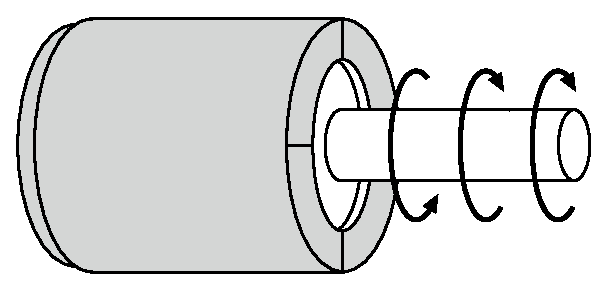
\includegraphics[width = 0.4\linewidth]{mechanical_diagram}};
            \begin{scope}[x={(image.south east)},y={(image.north west)}]
            %    \draw[help lines,xstep=.1,ystep=.1] (0,0) grid (1,1);
            %    \foreach \x in {0,1,...,9} { \node [anchor=north] at (\x/10,0) {0.\x}; }
            %    \foreach \y in {0,1,...,9} { \node [anchor=east] at (0,\y/10) {0.\y}; }
                \draw (0.7,0.125) node {$T_e$};
                \draw (0.82,0.85) node {$T_f$};
                \draw (0.95,0.85) node {$T_l$};
            \end{scope}
        \end{tikzpicture}
        \caption{Mechanical subsystem}
        \label{fig:mechanical_subsys}
    \end{figure}

    Applying Newton's second law to the motor's rotor, together with assumption \ref{hyp:rigid_bodies} we obtain the following equation

    \begin{equation}
        J.\frac{d^2\theta_m}{dt^2}=T_e-T_f-T_l,
        \label{eq:newtons_law_at_shaft}
    \end{equation}

    where $J$ is the motor's rotor inertia, $T_f$ is the resistance torque due to friction and $T_l$ is the torque applied by the load to the rotor.

    Because of \ref{hyp:friction_model}, $T_f$ can be decomposed as viscous friction (referred to as $T_{f1}$) and Coulomb friction (referred to as $T_{f2}$)

    \begin{equation}
        T_f = T_{f1} + T_{f2}.
    \end{equation}

    Viscous frictions can be calculated with

    \begin{equation}
        T_{f1} = K_d.\frac{d\theta_m}{dt},
    \end{equation}

    where $K_d$ is the damping constant.

    And Coulomb's model of friction [\textcolor{red}{citation needed}] is given by

    \begin{equation}
       T_{f2} = \left\{
         \begin{array}{lr}
           -T_k.sign(\frac{d\theta}{dt}) & : \frac{d\theta_m}{dt} \neq 0\\
           -min(T_s,T_e-T_l).sign(T_e-T_l) & : \frac{d\theta_m}{dt} = 0
         \end{array}
       \right.
       \label{eq:coulomb_friction_model}
    \end{equation}

    where $T_k$ is the static friction constant and $T_s$ is the kinetic friction constant.

    Analogously to section \ref{sec:elec_subsystem}, equations \ref{eq:newtons_law_at_shaft} through \ref{eq:coulomb_friction_model} model the dynamic relationship between the electromagnetic torque and the angular position of the rotor. This equations, together with equations \ref{eq:v_ab} through \ref{eq:total_torque}, constitute the full mathematical model used in the simulator.







\end{document}

